\documentclass[10pt]{article}

%Paquetes
\usepackage[utf8]{inputenc}
\usepackage{authblk}
\usepackage{graphicx}
\usepackage{mathtools}
\usepackage{geometry}
\usepackage{abstract}
\usepackage{multicol}



%comandos de formato
\renewcommand{\abstractname}{}
\renewcommand{\absnamepos}{empty}
\renewcommand{\thesection}{\Roman{section}} 
\renewcommand{\thesubsection}{\thesection.\Roman{subsection}}

\geometry{a4paper}
\geometry{margin=1in}
\addtolength{\topmargin}{-10mm}

%Encabezados
\title{\textbf{Hints on halo evolution in SFDM models with galaxy observations}}
\author[1]{Alma X. González-Morales}
\author[2]{Alberto Diez-Tejedor}
\author[2]{L. Arturo Ureña-López}
\author[3]{Octavio Valenzuela}

\affil[1]{\small Instituto  de  Ciencias  Nucleares,  Universidad  Nacional  Autónoma  de  Ḿexico,Circuito  Exterior  C.U.,  A.P.  70-543,  México  D.F.  04510,  México}
\affil[2]{\small Departamento  de  Física,  División  de  Ciencias  e  Ingenierías,Campus  León,  Universidad  de  Guanajuato,  León  37150,  México}
\affil[3]{\small Instituto  de  Astronomía,  Universidad  Nacional  Autónoma  de  México,Circuito  Exterior  C.U.,  A.P.  70-264,  México  D.F.  04510,  México\vspace{-2em}}

\date{(Dated: October 29, 2018)\vspace{-2em}}


%Inicio del documento
\begin{document}
\maketitle

\begin{abstract}\vspace{1em}
A massive, self-interacting scalar field has been considered as a possible candidate for the dark matter in the universe.  We present an observational constraint to the model arising from strong lensing observations in galaxies.  The result points to a discrepancy in the properties of scalar field dark matter halos for dwarf and lens galaxies, mainly because halo parameters are directly related to physical quantities in the model.  This is an important indication that it becomes necessary to have a better understanding of halo evolution in scalar field dark matter models, where the presence of baryons can play an important role.\\\\
PACS numbers:  95.30.Sf, 95.35.+d, 98.62.Gq, 98.62.Sb.
\end{abstract}


%Texto principal

\begin{multicols}{2}
\section{\large \centering INTRODUCTION}\\

The nature of dark matter (DM) remains elusive today,even though a generic cold particle weakly coupled to the standard model seems to be the most promising candidate \cite{Bertone_2005}.  Treating DM as a bunch of classical particles isan appropriate effective description for many physical sit-uations.  However, if DM is composed of bosons, the zero mode can develop a non-vanishing expectation value; this effect is usually known as Bose-Einstein condensation.  A condensed phase does not admit a description in terms of classical particles, and the concept of a coherent excitation (i.e.  a classical field) is more appropriate for practical purposes \cite{PhysRevD.28.1243}.  A specific realization of this scenario can be provided by the axion [3], see also [4].\\
In  this  paper  we  shall  explore  the  lensing  properties of a generic model of DM particles in a condensate, and compare the conditions necessary to produce strong lensing with those required to explain the dynamics of dwarf galaxies.  As a result we will get some insight into halo evolution arising from this type of models.\\
In  particular,  we  will  consider  the  case  of  a  complex,  massive,  self-interacting  scalar  field \(\phi \) satisfying the  Klein-Gordon (KG) equation, \(\phi - (mc/\hbar)^2 \phi - \lambda|\phi|^2\phi = 0\),with  the  box  denoting  the  d’Alembertian operator  in  four  dimensions.   For  those  natural  situations  in  which  the  scalar  field  massmis  much  smaller than  the  Planck  scale, \(m_{Plank}=(\hbar/c)^{1/2}\), such that \(\Lambda\equiv\lambda m_{Plank}^{2}/4\pi m^{2}\gg1\), the coherent (self-gravitating,spherically symmetric) solutions to the KG equation admit a very simple expression for the mass density [5, 6], 
\begin{equation} \label{eq:1}
		\rho(r)= \left\{ \begin{array}{lcc}
		\rho c\frac{\sin(\pi r/r_{max})}{(\pi r/r_{max})} 
		&   for  &   r< r_{max}
		\\ 0 &  for & r\geq r_{max} 
	\end{array} \right. 
\end{equation}

As usual we will refer to this model as scalar field dark matter (SFDM). Here \(r_{max}\equiv\sqrt{\pi^{2}\Lambda/2}(\hbar/mc)\) is a constant with dimensions of length (notice that \(r_{max}\) is just the  Compton  wavelength  of  the  scalar  particle,~/mc,scaled by a factor of order \(A^{1/2}\)), and \(\rho c\) he density at the center of the configuration.  The mass density profilein Eq. (\ref{eq:1}) leads to compact objects of size \(r_{max}\) and typical masses, \(4\rho r^{3}_{max}/\pi\) hat vary from configuration to configuration according to the value of the central den-sity.\\
Eq. (\ref{eq:1}) was obtained without taking into account thegravitational influence of any other matter sources, andassuming that all the scalar particles are in the conden-sate.  It has been used as a first order approximation todescribe the distribution of matter in dwarf shperoidals,which are expected to be DM dominated [6–8].  The massdistribution would be smooth close to the center of thesegalaxies, alleviating the cusp/core problem motivated bythe  discrepancies  between  the  observed  high  resolutionrotation curves and the profiles suggested by N-body sim-ulations [9]; see however [10].\\

The   dynamics   of   dwarf   galaxies   suggests   a   self-interacting  scalar  with \(m^{4}/\lambda\sim50-75(eV)^{4}\) (i.e. \( r_{max}\sim5.5-7Kco\)) , and typical central densities of theorder of \(\rho c\sim10^{-3}M_{\odot}/pc^{3}\)see Ref. [6].  We are awarethat  Milky  Way  size  galaxies  are,  at  least,  an  order  ofmagnitude larger than this value of \(r_{max}\)and then theydo  not  fit  in  this  model  as  it  stands.   Nonetheless,  ifnot all the DM particles are in the condensate, there isa  possibility  to  have  gravitational  configurations  wherethe inner regions are still described by the mass densityprofile in Eq.  (\ref{eq:1}), wrapped in a cloud of non-condensedparticles [11].  For the purpose of this paper we do notneed to specify the complete halo model.  This is becausestrong lensing is not very sensitive to the mass distribu-tion outside the Einstein radius, at most of the order ofa few Kpc, just bellow the expected value of \(r_{max}\)Wecould not neglect the exterior profile of the halo if we wereinterested, for instance, in weak lensing observations.

\section{\large \centering LENSING PROPERTIES OF SFDM HALOS}\\

In  the  weak  field  limit  the  gravitational  lensing  pro-duced by a mass distribution can be read directly fromthe density profile.  As usual we assume spherical symme-try, and use the thin lens approximation, that is, the sizeof  the  object  is  negligible  when  compared  to  the  otherlength scales in the configuration, i.e.  the (angular) dis-tances between the observer and the lens,,DOL, the lensand the source,DLS, and from the observer to the source,DOS.\\
	Under these assumptions the lens equation takes theform \\
	\begin{equation}\label{eq:2}
		\beta=\theta-\frac{M(\theta)}{\pi D^{2}{OL}\theta\sum{cr}},
	\end{equation}
	
whit \(\beta\) and \(\theta\) enoting the actual (unobservable) angularposition of the source, and the apparent (observable) an-gular position of the image, respectively, both measuredwith  respect  to  the  line-of-sight  [12].   The  (projected)mass  enclosed  in  a  circle  of  radius \(\xi\),\(M (\xi)\), s  definedfrom the (projected) surface mass density, \(\sum(\xi)\) through,\\
   \begin{equation}\label{eq:3}
   	\sum(\xi)\equiv\int_{-\propto}^{\propto}dz \rho(z,\xi), \\ M(\xi)\equiv2\pi\int_{0}^{\xi}d\xi\prime\xi\prime\sum(\xi\prime)
   \end{equation}\\
   
Here \(\xi=D_{OL}\theta\) In general, Eq. (\ref{eq:2}) will be non-linear in \(\theta\), and it couldbe possible that for a given position of the source,\(\beta\), therewould  be  multiple  solutions  (i.e.   multiple  images)  forthe angle \(\theta\).  This is what happens in the strong lensingregime to be discussed below.  One particular case is thatwith a perfect alignment between the source and the lens,that actually defines the Einstein ring, with an angularradius of \(\theta E \equiv \theta(\beta=0)\).\\
For  a  SFDM  halo,  and  in  terms  of  the  normalized lengths \(\xi_{}\equiv \xi/ r_{max}\) and \(z_{}\equiv z/r_{max}\) he surface massdensity takes the form.\\
\begin{equation}\label{eq:4} 
	\sum SFDM(\xi_{}) = \frac{2 \rho_{c} r_{max}}{\pi} \int_{0}^{z_{max}}\frac{\sin(\pi \sqrt{\xi^{2}_{}+z^{2}_{}})}{\sqrt{\xi^{2}_{}+z^{2}_{*}}} 
\end{equation}\\

wirh \(0\leq \xi_{}\leq 1 \) and \(z_{max} = \sqrt{1-\xi^{2}_{}}\). A  similarexpression  can  be  obtained  for  the  mass  enclosed  in  acircle  or  radius \(\xi\) see  Eq.   (\ref{eq:3})  above.   Here  we  are  notconsidering the effect of a scalar cloud surrounding thecondensate.  For \(r \leq r_{max}\) his will appear as a projectioneffect,  which is usually considered to be small \cite{Kling_2008}.  In-deed, we have corroborated that the inclusion of an outerisothermal sphere does not affect the conclusions of thispaper.With the use of the expression for the projected mass,\(M_{SFDM}(\xi_{*})\) he lens equation simplifies to
\begin{equation}\label{5a}
	\beta_{}(\theta_{})=\theta_{}-\bar{\lambda} \frac{m(\theta_{})}{\theta_{*}}
\end{equation}

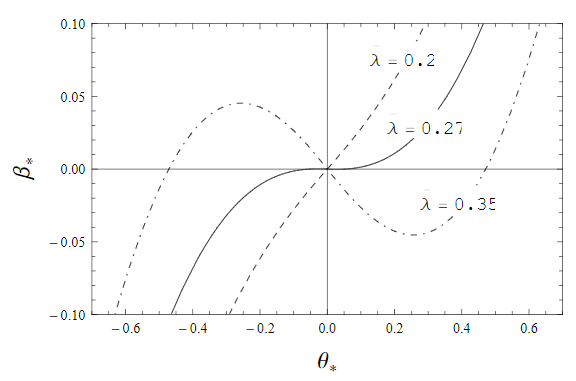
\includegraphics[width=7cm]{fig1.png} \label{fig:1}
FIG. 1.  The lens equation of a SFDM halo model, Eq.  (\ref{5a}), as a function of \(\bar{\lambda}\) The roots define the Einstein radius, \(\theta_{*E}\)E, andits local maximum (minimum) the critical impact parameter, \(\beta_{*cr}\) Both quantities are well defined only for values of \(\bar{\lambda}>\bar{\lambda}_{cr}\simeq0.27\) , which is the threshold value for strong lensing.

where \(m(\xi_{})\equiv M_{SFDM}(\xi_{})/\rho_{c}r_{max}^{3}\) is a normalized massfunction, evaluated numerically.  Here \(\beta_{}=D_{OL}\beta/r_{max}\) and \(\theta_{}=D_{OL}\theta/r_{max}\) are  the  normalized  angular  posi-tions of the source and images, respectively, and the parameter \(\bar{\lambda}\)\\
\begin{equation}\tag{5b}
	\bar{\lambda}\equiv\frac{\rho_{c}r_{max}}{\pi\sum_{cr}}=0.57\hbar^{-1}(\frac{\rho_{c}}{M_{\odot}pc^{-3}})(\frac{r_{max}}{kcp})\frac{d_{OL}d_{LS}}{d_{OS}} 
\end{equation}

In order to avoid confusion with the self-interaction term, \(\lambda\), we have introduced a bar in the new parameter \(\bar{\lambda}\) .  Wehave  also  defined  the  reduced  angular  distances \(d_{a}\equiv D_{A}H_{0}/c\), and considered \(H_{0} \equiv 100 \hbar (km/s)/Mpe\) as the Hubble constant today, with \(h=0.710 \pm 0.025\) [14].In Fig. \ref{fig:1} we show the behavior of the lens equation (\ref{5a}) as the \(\bar{\lambda}\) parameter varies (i.e.  for different values of the combination \(\rho_{c} r_{max}\) ).  Some notes are in turn:i) Stronglensing can be produced only for configurations with \(\bar{\lambda} > \bar{\lambda}{cr}\simeq 0.27\), andii) For these configurations, only thosewith an impact parameter \(|\beta{*}|<\beta_{*cr}\) can produce threeimages (note that the actual value of \(\beta_{*cr}\) depends on theparameter \(\bar{\lambda}\), \(\beta_{*cr}(\bar{\lambda})\)). 

These conditions on the SFDM profile are very similarto those obtained for the Burkert model in \cite{Park_2003}; this is notsurprising because both of them have a core in radius.  Inthat sense SFDM halos are analogous to those proposedby Burkert \cite{Burkert_1995}, but with the advantage that their prop-erties are clearly connected to physical parameters in themodel.

In  Fig.  \ref{fig:2}  we  show  the  magnitude  of  the  Einstein  radius, \(\theta_{*E}\),  as  a  function  of  the  paramete \(\bar{\lambda}\) ,  where  forcomparison we have also plotted the same quantity forthe NFW [17] and Burkert [15] profiles.  The minimumvalue of \(\bar{\lambda}\) needed to produce multiple images is higher fora SFDM halo \(\bar{\lambda}{cr}^{NFW} = 0 < \bar{\lambda}{er}^{Burkert} = 2/\pi^{2} < \bar{\lambda}_{cr}^{SFDM} \simeq 0.27 \) .   (Notice  that  there  is  an  extra  factor  of \(1/4\pi\) inour  definition  of \(\bar{\lambda}\) when  compared  to  that  reported  inRef. [15].)  SFDM halos seem to require larger values of \\

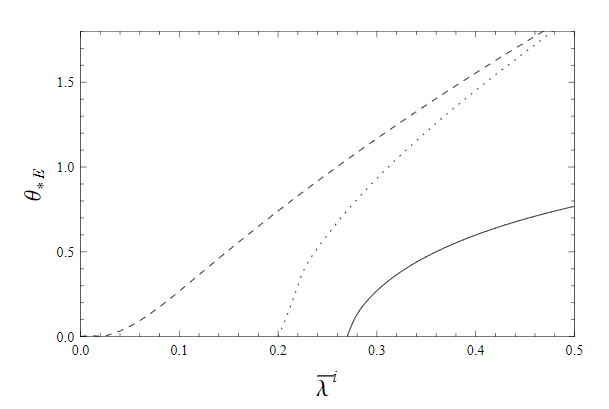
\includegraphics[width=7cm]{fig2.png}\label{fig:2}
FIG. 2 The  Einstein  radius, \(\theta_{*E}\)  as  function  of \(\bar{\lambda}^{i}\) forSFDM (solid line), NFW (dashed line), and Burkert (dottedline) halo models.  Einstein rings of similar magnitude require \(\bar{\lambda}^{NFW}<\bar{\lambda}^{Burkert}<\bar{\lambda}^{SFDM}\). 
 
\(\bar{\lambda}\) in order to produce Einstein rings of similar magnitudeto those obtained for the other profiles, but this is in partdue to projection effects that have not been consideredin this paper [13, 18].

\section{\large \centering LENSING VS DYNAMICS}\\

Taking into account that in SFDM models there is acritical value for the parameter \(\bar{\lambda} , \bar{\lambda}_{cr} \simeq .027\), and con-sidering the definition in Eq. (\ref{5a}), we can write the con-dition to produce strong lensing in the form \\
\begin{equation}\label{eq:6}
	\rho_{c} r_{max}[M_{\odot}pc^{-2}]  < 473.68 \hbar f_{dist}
\end{equation}

with \(f_{dist}\equiv d_{OS}/d_{OL}d_{LS}\) a distance factor.In  order  to  evaluate  the  right-hand-side  (r.h.s.)    of Eq. (\ref{eq:6}), we consider two surveys of multiply-imaged sys-tems,  the  CASTLES  [19]  and  the  SLACS  [20].   Fromthem  we  select  only  those  elements  for  which  the  red-shifts  of  the  source  and  the  lens  have  been  determined(which  amounts  to  approximately  60  elements  in  eachsurvey),  and  calculate  the  corresponding  distance  fac-torfdistfor  every  element  in  the  reduced  sample.   InCASTLES (SLACS) the distance factors are in the interval  \(4<f_{dist}<27, (6<f_{dist})<25\), with a mean value of \(f_{dist}\simeq 7, (f_{dist}\simeq 11)\), and then the r.h.s.  of Eq. (\ref{eq:6})takes on values in the range \(1400-9000, (2000-8500)\).Some representative elements from SLACS are shown inTable  I  (galaxy  lensing).   In  terms  of  the  mean  values,the inequality in Eq. (\ref{eq:6}) translates into
 \begin{equation}\label{eq:7a}
 	\rho_{c}r_{max}[M_{\odot}pc^{-2}]>2000, (CASTLES)
 \end{equation}
  \begin{equation}\label{7b}
 	\rho_{c}r_{max}[M_{\odot}pc^{-2}]>4000, (SLACS)
 \end{equation}
 
These  numbers  are  an  order  of  magnitude  greaterthan   those   obtained   from   dwarf   galaxies   dynamics, \(\rho_{C}r_{max}[M_{\odot}]\simeq 100\), , when interpreted using the samedensity profile [7]; see again Table I. This is the main re-sult of the paper.  Remember that the value of \(r_{max}\) is re-lated to the fundamental parameters of the model, which are the mass of the scalar particle and the self-interactionterm, and it remains constant throughout the formationof cosmic structure.We must recall that inequalities in Eq.  (\ref{eq:7a}) do not takeinto account the presence of baryons in galaxies.  Gravitydoes not distinguish between luminous and dark matter;then the contribution of the former to the lens could besignificant in some cases.  For instance, for those systemsin SLACS the stellar mass fraction within the Einsteinradius is 0.4, on average, with a scatter of 0.1 [21].We have corroborated that our estimates in Eq. (\ref{eq:7a}) arenot sensitive to the inclusion of a baryonic component.To  see  that  we  add  the  contribution  of  a  de  Vacoulersurface brightness profile [22] to the lens equation,
\begin{equation}\label{eq:8a}
	\beta_{}(\theta_{})=\theta_{}-\bar{\lambda} \frac{m(\theta_{})}{\theta_{}}-\bar{\lambda}{lum} \frac{f(\theta{}/r_{e*})}{\theta_{*}}
\end{equation}

 Here \(\bar\lambda\) is  a  parameter  analogous  to  that  given  inEq (5b),
\begin{equation}\tag{8b}
	\bar{\lambda}{lum}\equiv \frac{(M/L)M}{2\pi\sum{cr}}, 
\end{equation} 

and f(x) a dimensionless projected stellar mass,
\begin{multline*}\tag{8c}
	 f(x)=\frac{1}{2520}[e^{q}(q^{7}-7q^{6}+42q^{5}-210q^{4}+840q^{3} \\ -2520q^{2}+5040q-5040)+5040],
\end{multline*}

with \(q\equiv -7.76x^{-1/4}\). he  mass-to-light  ratio, M/L(from  a  Chabrier  initial  mass  function),  and  the  effec-tive radius, \(r_{e}\),for each system in SLACS are reportedin Ref. [21].  With the use of Eq.  (\ref{eq:8}) strong lensing is al-ways possible.  Consequently, we must impose a differentcondition to constrain the product, \(\rho_{c}r_{max}\) in each galaxy,such as demand the formation of Einstein rings of certainradius.

o proceed we use a small subsample of SLACS that in-cludes configurations with the minimum, maximum, andmean  Einstein  radius,  and  stellar  surface  mass  density,respectively.  This is because the new lens equation is afunction of the ratio \(r_{e*}=r_{e}/r_{max}\); then, to compute themagnitudes of the Einstein radii, we shall fix the value of \(r_{max}\) a priori. 

Using the new lens equation we find the value of \(\bar{\lambda}\) thatproduces the appropriate Einstein radius for each of theelements in the subsample.  This is done using two differ-ent values of \(r_{max}\):5 and 10 Kpc.  The resultant products \(\rho_{c}r_{max}\) are compatible (in order of magnitude) with theinequalities obtained from Eq.  (\ref{eq:6}).  Only for those sys-tems in the subsample with a high stellar surface massdensity  the  value  of \(\rho_{c}r_{max}\) can  decrease  substantially,but it is important to have in mind that all the possibleuncertainties associated to the distribution of the lumi-nous  matter,  like  the  choice  of  the  stellar  initial  massfunction,  will  be  more  relevant  in  such  cases.   In  gen-eral, these estimations are sensitive to the details of theparticular  configuration,  and  a  more  exhaustive  analy-sis,  considering  the  complete  sample,  will  be  presented elsewhere.

\end{multicols}

\begin{table}[h!]
	\centering
	\begin{tabular}{|l|l|l|l|l|} 
		\hline
		\multicolumn{2}{|l|}{\textbf{\centering DINAMICS OF GALAXIES}} & \multicolumn{3}{l|}{\textbf{\centering GALAXY LENSING}}  \\ 
		\hline
		Galaxy     & \(\rho_{C}r_{max}[M_{\odot}pc^{-2}]\)                          & Galaxy     & fdist & \(\rho_{C}r_{max}[M_{\odot}pc^{-2}]\)              \\ 
		\hline
		Ho II      & 36.19                         & J0008-0004 & 6.16  & 2029.68         \\ 
		\hline
		DDO 154    & 66.46                         & J1250+0523 & 8.46  & 28320.41        \\ 
		\hline
		DDO 53     & 67.53                         & J2341+0000 & 9.12  & 3053.38         \\ 
		\hline
		IC2574     & 81.89                         & J1538+5817 & 11.74 & 3930.44         \\ 
		\hline
		NGC2366    & 85.45                         & J0216-0813 & 13.03 & 4362.44         \\ 
		\hline
		Ursa Minor & 104.72                        & J1106+5228 & 15.74 & 5269.75         \\ 
		\hline
		Ho I       & 120.23                        & J2321-0939 & 16.23 & 54433.8         \\ 
		\hline
		DDO 39     & 145.94                        & J1420+6019 & 19.72 & 6602.26         \\ 
		\hline
		M81 dwB    & 265.87                        & J0044+0113 & 25.26 & 8457.05         \\
		\hline
	\end{tabular}
\end{table} \label{table:1}
TABLE  I.   Estimates  of  the  productρcrmaxfor  different  galaxies.Left.As  reported  in  Refs.   [7],  using  galactic  dynamics.Right.Derived from equation (6) in this paper; recall that these values represent a lower limit (here we show only a representativesubsample of the SLACS survey).  Note the difference of an order of magnitude between the values ofρcrmaxfor dwarf galaxiesin the local universe, and the lower limit of this same quantity for galaxies producing strong lensing atz∼0.5.\\



\begin{multicols}{2}

\section{\large \centering DISCUSSION AND FINAL REMARKS}\\

We have shown that a discrepancy between lensing anddynamical studies appears if we consider that the SFDMmass density profile in Eq. (1) describes the inner regionsof galactic halos at different redshifts, up to radii of order5−10 Kpc.   More  specifically,  we  have  found  that  lensgalaxies atz∼0.5, if correctly described by a SFDM haloprofile,  should  be  denser  than  dwarf  spheroidals  in  thelocal universe, in order to satisfy the conditions necessaryto produce strong lensing.In  principle  nothing  guarantees  that  halos  of  differ-ent kind of galaxies share the same physical properties.Our  studies  took  into  account  galaxies  that  are  intrin-sically different in terms of their total mass and baryonconcentration.  While dwarf galaxies show low stellar sur-face brightness, stellar component in massive, early typegalaxies is typically compact and dense.In  the  standard  cosmological  model  the  evolution  ofDM  halos  may  trigger  differences  in  concentrations  forhalos with different masses due to differences in the as-sembling epoch; smaller halos collapsed in an earlier anddenser universe, therefore they are expected to be moreconcentrated.   However,  it  is  also  well  known  that  thepresence of baryons during the assembly of galaxies canalter  the  density  profile  of  the  host  halos  and  modifythis  tendency,  making  them  shallower  (supernova  feed-back  [23]),  or  even  cuspier  (adiabatic  contraction  [24]).Therefore,  the  stellar  distribution  may  reveal  differentdynamical  evolution  for  low  and  high  mass  halos  trig-gered by galaxy formation.For SFDM, the dynamical interaction between baryonsand  the  scalar  field  may  also  modify the  internal  halostructure predicted by the model, Eq. (1), clarifying thediscrepancy.   For  instance,  if  the  concentration  of  stel-lar  distribution  were  correlated  with  that  of  the  halo,like in the adiabatic contraction model when applied tostandard DM halos, this may explain our findings.  Butat this time it is unknown how compressible SFDM ha-los are, and if such effect will be enough to explain ourresults,  because  there  are  no  predictions  on  its  magni-tude. If the modification triggered by baryons were insuf-ficient, then it might be suggesting an intrinsic evolutionof SFDM halos across cosmic time.  For example, if biggalaxies  emerge  as  the  result  of  the  collision  of  smallerones, then the central densities of the resultant galaxieswould be naturally higher;  after all,rmaxis a constantin  the  model,  and  one  would  expect  that  total  mass  ispreserved in galaxy-galaxy mergers.  At this point we donot know which of these two mechanisms, the intrinsic tothe model, or that due to the evolution of SFDM halosin the presence of baryons, is the dominant one.  In thatsense, a theoretical description of these processes may bevery useful and welcome.A full picture requires a distribution of values for thecentral density generated from the evolution of the spec-trum of primordial density perturbations after inflation.Such a result is not available now,  but it is possible tostart tracing this distribution with galaxy observations.We present, for the first time, observational constraintson the dynamical evolution of SFDM halos in the pres-ence of baryons, that must be considered for future semi-analytical/numerical studies of galaxy formation.

\section*{\large \centering ACKNOWLEDGEMENTS}\\

We are grateful to Juan Barranco for useful comments.This work was partially supported by PROMEP, DAIP-UG, CAIP-UG, PIFI, I0101/131/07 C-234/07 of the In-stituto  Avanzado  de  Cosmologia  (IAC)  collaboration,DGAPA-UNAM  grant  No.   IN115311,  and  CONACyTM ́exico  under  grants  167335,  182445.   AXGM  is  verygrateful to the members of the Departamento de F ́ısicaat Universidad de Guanajuato for their hospitality.

\end{multicols}

\begin{multicols}{2}

\bibliographystyle{plain}
\bibliography{referencias.bib}

\end{multicols}

\end{document}